% Copyright (c) anneal developers
\documentclass[aip,jcp,preprint,amsmath,amssymb]{revtex4-2}
\usepackage{graphicx,booktabs,longtable}
\graphicspath{{figs/}{../jctc/figs/}}

\begin{document}
\title{Supplementary material: Basin hopping for atomic clusters with a fixed move library}
\author{Rohit Goswami}
\affiliation{SURF B.V., Amsterdam, The Netherlands}
\maketitle

\section{Rank weights}
The campaigns in the article use \(T=0.8\,\varepsilon\).
A population can instead be reweighted by within-epoch ranks.
In a population of \(R\ge 2\), a tied block from \(b\) inclusive to \(e\) exclusive has rank
\begin{equation}
r=(b+e-1)/(2(R-1)).
\end{equation}
The energy, novelty, scarcity and uncertainty ranks combine as
\begin{equation}
\log w_i=-r_{E,i}+0.8\,r_{N,i}+0.6\,r_{S,i}+0.4\,r_{U,i}.
\end{equation}
The coefficients are those of the communicating-chain account.\cite{goswami2023}
A bank is communicating when each chain draws its move from a depth posterior, a packing retires on the Good-Turing mass, minima are merged at one radial distance, every force call is charged to the chain that spent it, and a receiver may quench a shared minimum.
Parallel tempering, population annealing, conformational space annealing and cut-and-splice are the neighbouring constructions.\cite{swendsenReplicaMonteCarlo1986,hukushimaExchangeMonteCarlo1996,hukushimaPopulationAnnealingIts2003,machtaPopulationAnnealingWeighted2010,leeUnbiasedGlobalOptimization2003,deaven1995,geudtner2025}

\section{Oakley means}
Means below are over runs that continued until success, with no call cap.\cite{oakley2013}
Continuous-symmetry basin hopping at 38 atoms averages 4369 evaluations over 100 runs.
Core-orbit basin hopping at 75 atoms averages 50229 evaluations over 100 runs.
Core-orbit genetic-algorithm means are 87250 at 75 atoms and 178651 at 98 atoms.

\section{Sixty-four seed campaign}
{\scriptsize
\begin{longtable}{llrrrr}
\caption{Earlier multi-code campaign. A blank call median was withheld in the source table. TIP4P with 20 molecules has 16 seeds. Every other row has 64.\label{tab:campaign}}\\
\toprule
System & Code & Hits & Call median & Wall median (s) & Cores \\
\midrule\endfirsthead
\toprule System & Code & Hits & Call median & Wall median (s) & Cores \\
\midrule\endhead
\bottomrule\endlastfoot
lj38 & anneal-rec & 64/64 & 722.5 & 0.005791324999972255 & 1\\
lj38 & anneal-lean & 64/64 & 5332.0 & 0.0975008780004335 & 1\\
lj38 & anneal-full & 64/64 & 5839.5 & 0.09116734199996918 & 1\\
lj38 & anneal-ens & 64/64 & --- & 0.6610531444996556 & 1\\
lj38 & anneal-dls & 53/64 & --- & 1.8097005875000893 & 1\\
lj38 & gmin-bh & 64/64 & 3638.0 & 0.0443917180000426 & 1\\
lj38 & gmin-sym & 64/64 & 21647.0 & 0.19107757150004545 & 1\\
lj38 & gmin-bhpt & 55/64 & --- & 1.1142728230001921 & 4\\
lj38 & ogolem & 54/64 & 596657.5 & 8.54352395100068 & 1\\
lj38 & abcluster & 22/64 & 2400000.0 & 22.310232143000576 & 1\\
lj55 & anneal-rec & 64/64 & 10094.0 & 0.2824030050000877 & 1\\
lj55 & anneal-full & 64/64 & 9552.0 & 0.3234629180001056 & 1\\
lj55 & anneal-ens & 64/64 & --- & 0.27568861200035216 & 1\\
lj55 & anneal-dls & 58/64 & --- & 0.3115833569999432 & 1\\
lj55 & gmin-bh & 62/64 & 15931.0 & 0.26193437700021605 & 1\\
lj55 & gmin-bhpt & 63/64 & --- & 0.45282894999991186 & 4\\
lj55 & ogolem & 64/64 & 53229.5 & 5.5159799534999365 & 1\\
lj55 & abcluster & 46/64 & 22153.0 & 0.37575116949983567 & 1\\
lj75 & anneal-rec & 64/64 & 25394.5 & 1.335708618500296 & 1\\
lj75 & anneal-full & 64/64 & 30128.0 & 1.721641731000028 & 1\\
lj75 & anneal-ens & 20/64 & --- & 11.150663114000963 & 1\\
lj75 & anneal-dls & 0/64 & --- & 10.752445379999699 & 1\\
lj75 & gmin-bh & 63/64 & 38350.0 & 1.5508648014997561 & 1\\
lj75 & gmin-bhpt & 0/64 & --- & 8.045407886000248 & 4\\
lj75 & ogolem & 0/64 & 800000.0 & 23.972671633999198 & 1\\
lj75 & abcluster & 0/64 & 800000.0 & 22.137346516000434 & 1\\
lj98 & anneal-rec & 36/64 & 824807.0 & 85.41052182900017 & 1\\
lj98 & anneal-full & 27/64 & 2000000.0 & 198.46848655699796 & 1\\
lj98 & anneal-ens & 59/64 & --- & 9.27265536399996 & 1\\
lj98 & anneal-dls & 29/64 & --- & 42.305233376000615 & 1\\
lj98 & gmin-bh & 61/64 & 321201.5 & 14.560340063500007 & 1\\
lj98 & gmin-bhpt & 1/64 & --- & 33.38894520899976 & 4\\
lj98 & ogolem & 2/64 & 2000000.0 & 53.56404115800069 & 1\\
lj98 & abcluster & 0/64 & 2000000.0 & 90.98174912100149 & 1\\
lj104 & anneal-rec & 0/64 & 2000000.0 & 218.98200713000006 & 1\\
lj104 & anneal-full & 0/64 & 2000000.0 & 239.25476196599993 & 1\\
lj104 & anneal-ens & 36/64 & --- & 19.558123004499624 & 1\\
lj104 & anneal-dls & 1/64 & --- & 49.279001113999584 & 1\\
lj104 & gmin-bh & 0/64 & 2000000.0 & 148.63462204000098 & 1\\
lj104 & gmin-bhpt & 1/64 & --- & 37.657022895999944 & 4\\
lj104 & ogolem & 6/64 & 2000000.0 & 56.72625435700047 & 1\\
lj104 & abcluster & 0/64 & 2000000.0 & 101.94683742300003 & 1\\
tip4p10 & anneal-rec & 64/64 & 10773.0 & 0.047659832500148304 & 1\\
tip4p10 & anneal-full & 64/64 & 9802.5 & 0.046492630500106095 & 1\\
tip4p10 & gmin-bh & 64/64 & 11616.0 & 0.1170010989999355 & 1\\
tip4p10 & gmin-tbp & 64/64 & 13164.0 & 0.13375579349985856 & 1\\
tip4p10 & abcluster & 30/64 & 400000.0 & 3.449306918999355 & 1\\
tip4p15 & anneal-rec & 0/64 & 10400000.0 & 107.52276586299922 & 1\\
tip4p15 & anneal-full & 2/64 & 10400000.0 & 120.98977565899986 & 1\\
tip4p15 & gmin-bh & 64/64 & 618020.0 & 13.391472141999657 & 1\\
tip4p15 & gmin-tbp & 64/64 & 378559.0 & 8.904109952999988 & 1\\
tip4p15 & abcluster & 8/64 & 10400000.0 & 183.09601579399896 & 1\\
tip4p20 & anneal-rec & 0/16 & 60000000.0 & 1904.153756404001 & 1\\
tip4p20 & anneal-full & 1/16 & 60000000.0 & 1424.8577746479968 & 1\\
tip4p20 & gmin-bh & 8/16 & 41091439.0 & 1422.7759169104975 & 1\\
tip4p20 & gmin-tbp & 10/16 & 15760138.0 & 552.056812917499 & 1\\
tip4p20 & abcluster & 0/16 & 60000000.0 & 1693.1663264809977 & 1\\
\end{longtable}

}

The paired full arm hits 24/64 on \(\mathrm{LJ}_{98}\) against 64/64 for GMIN.
The median paired call ratio is 12.62, and 2000 resamples give 8.52--15.22.
On \(\mathrm{LJ}_{55}\) that arm hits 63/64 and GMIN hits 64/64.
Plain basin hopping hits 26/64 and 7/64.
ABCluster hits 64/64 and 1/64.
In the family of these six comparisons, the Holm-adjusted McNemar and Wilcoxon tests below 0.05 are the \(\mathrm{LJ}_{98}\) comparisons of the full arm, plain basin hopping and ABCluster with GMIN, and the \(\mathrm{LJ}_{55}\) comparison of plain basin hopping with GMIN.

\section{Hexamer counters}
\begin{table}
\caption{CREST effort on the water hexamer.
The energy-and-gradient column is the cost in the article.}
\begin{ruledtabular}
\begin{tabular}{crr}
Seed & Dynamics + optimisation & Energy and gradient \\
\hline
0 & 32112 & 151074 \\
1 & 50026 & 191132 \\
2 & 32155 & 142110 \\
3 & 46062 & 172468 \\
4 & 50063 & 157643 \\
5 & 32170 & 209931 \\
\end{tabular}
\end{ruledtabular}
\end{table}

\section{TIP4P constants}
Jorgensen's pair is \(A=2510400\,\mathrm{kJ\,mol^{-1}\,\text{\AA}^{12}}\) and \(C=2552.24\,\mathrm{kJ\,mol^{-1}\,\text{\AA}^{6}}\).\cite{jorgensen1983}
GMIN stores these as \(C_{12}\) and \(C_6\).
The anneal rows use \(\varepsilon=0.6485\,\mathrm{kJ\,mol^{-1}}\) and \(\sigma=3.15365\,\text{\AA}\), giving \(C_6=2551.8252\) and \(C_{12}=2510336.2\).
The relative difference is \(-3.0\times 10^{-4}\) in the well depth and \(2.3\times 10^{-5}\) in \(\sigma\).

\section{Gupta clusters and the Cu--H slab}
\begin{table}
\caption{Gupta zinc and Cu\(_{19}\)Au\(_{19}\).
The ratio is the ASE median wall divided by the anneal median wall.}
\begin{ruledtabular}
\begin{tabular}{llrrrr}
System & Arm & Hits & Budget & Wall (s) & Ratio \\
\hline
Zn\(_{38}\) & anneal & 1/6 & 50000 & 1.285 & 183 \\
Zn\(_{38}\) & ASE & 2/6 & 50000 & 235.3 & 183 \\
Zn\(_{55}\) & anneal & 0/6 & 80000 & 4.542 & 169 \\
Zn\(_{55}\) & ASE & 0/6 & 80000 & 768.1 & 169 \\
Zn\(_{75}\) & anneal & 0/6 & 100000 & 11.32 & 147 \\
Zn\(_{75}\) & ASE & 0/6 & 100000 & 1659 & 147 \\
Zn\(_{80}\) & anneal & 0/6 & 100000 & 13.24 & 158 \\
Zn\(_{80}\) & ASE & 0/6 & 100000 & 2093 & 158 \\
Cu\(_{19}\)Au\(_{19}\) & anneal & 0/6 & 80000 & 4.012 & 141 \\
Cu\(_{19}\)Au\(_{19}\) & ASE & 0/6 & 80000 & 565.8 & 141 \\
\end{tabular}
\end{ruledtabular}
\end{table}

Eight seeds on the FCC Cu--H slab, reference \(-415.971529\,\mathrm{eV}\), all lie inside \(0.001\,\mathrm{eV}\).
Best energies run from \(-415.971521\,\mathrm{eV}\) to \(-415.971161\,\mathrm{eV}\).
Gaps above the reference run from \(8\times 10^{-6}\,\mathrm{eV}\) to \(3.68\times 10^{-4}\,\mathrm{eV}\).

\section{Plates and maps}
\begin{figure}
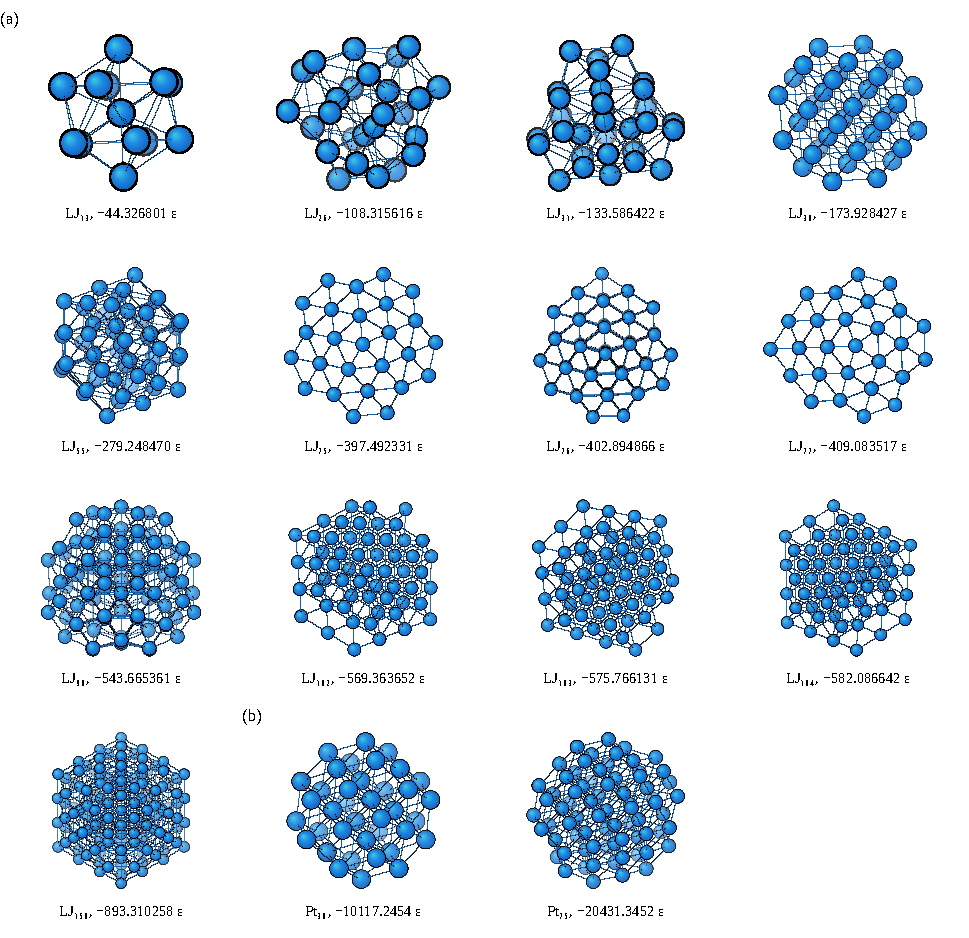
\includegraphics[width=\textwidth]{si_structures.pdf}
\caption{Reference geometries used to draw the benchmark.}
\end{figure}
\begin{figure}
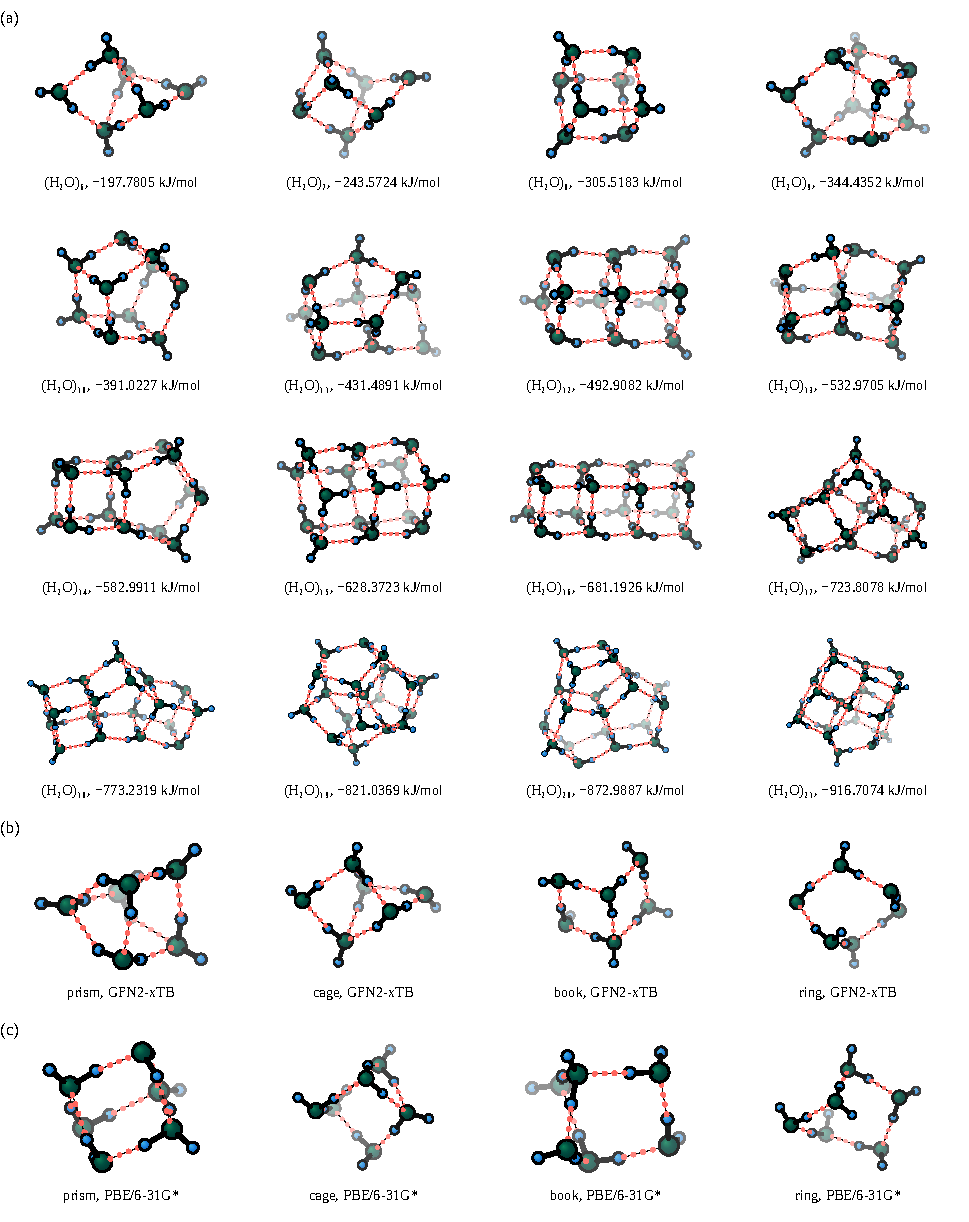
\includegraphics[width=\textwidth]{si_water.pdf}
\caption{Water plates.
The printed hexamer energy, \(-197.7805\,\mathrm{kJ\,mol^{-1}}\), is the TIP4P Cambridge value on Jorgensen's \(A\) and \(C\).}
\end{figure}
\begin{figure}
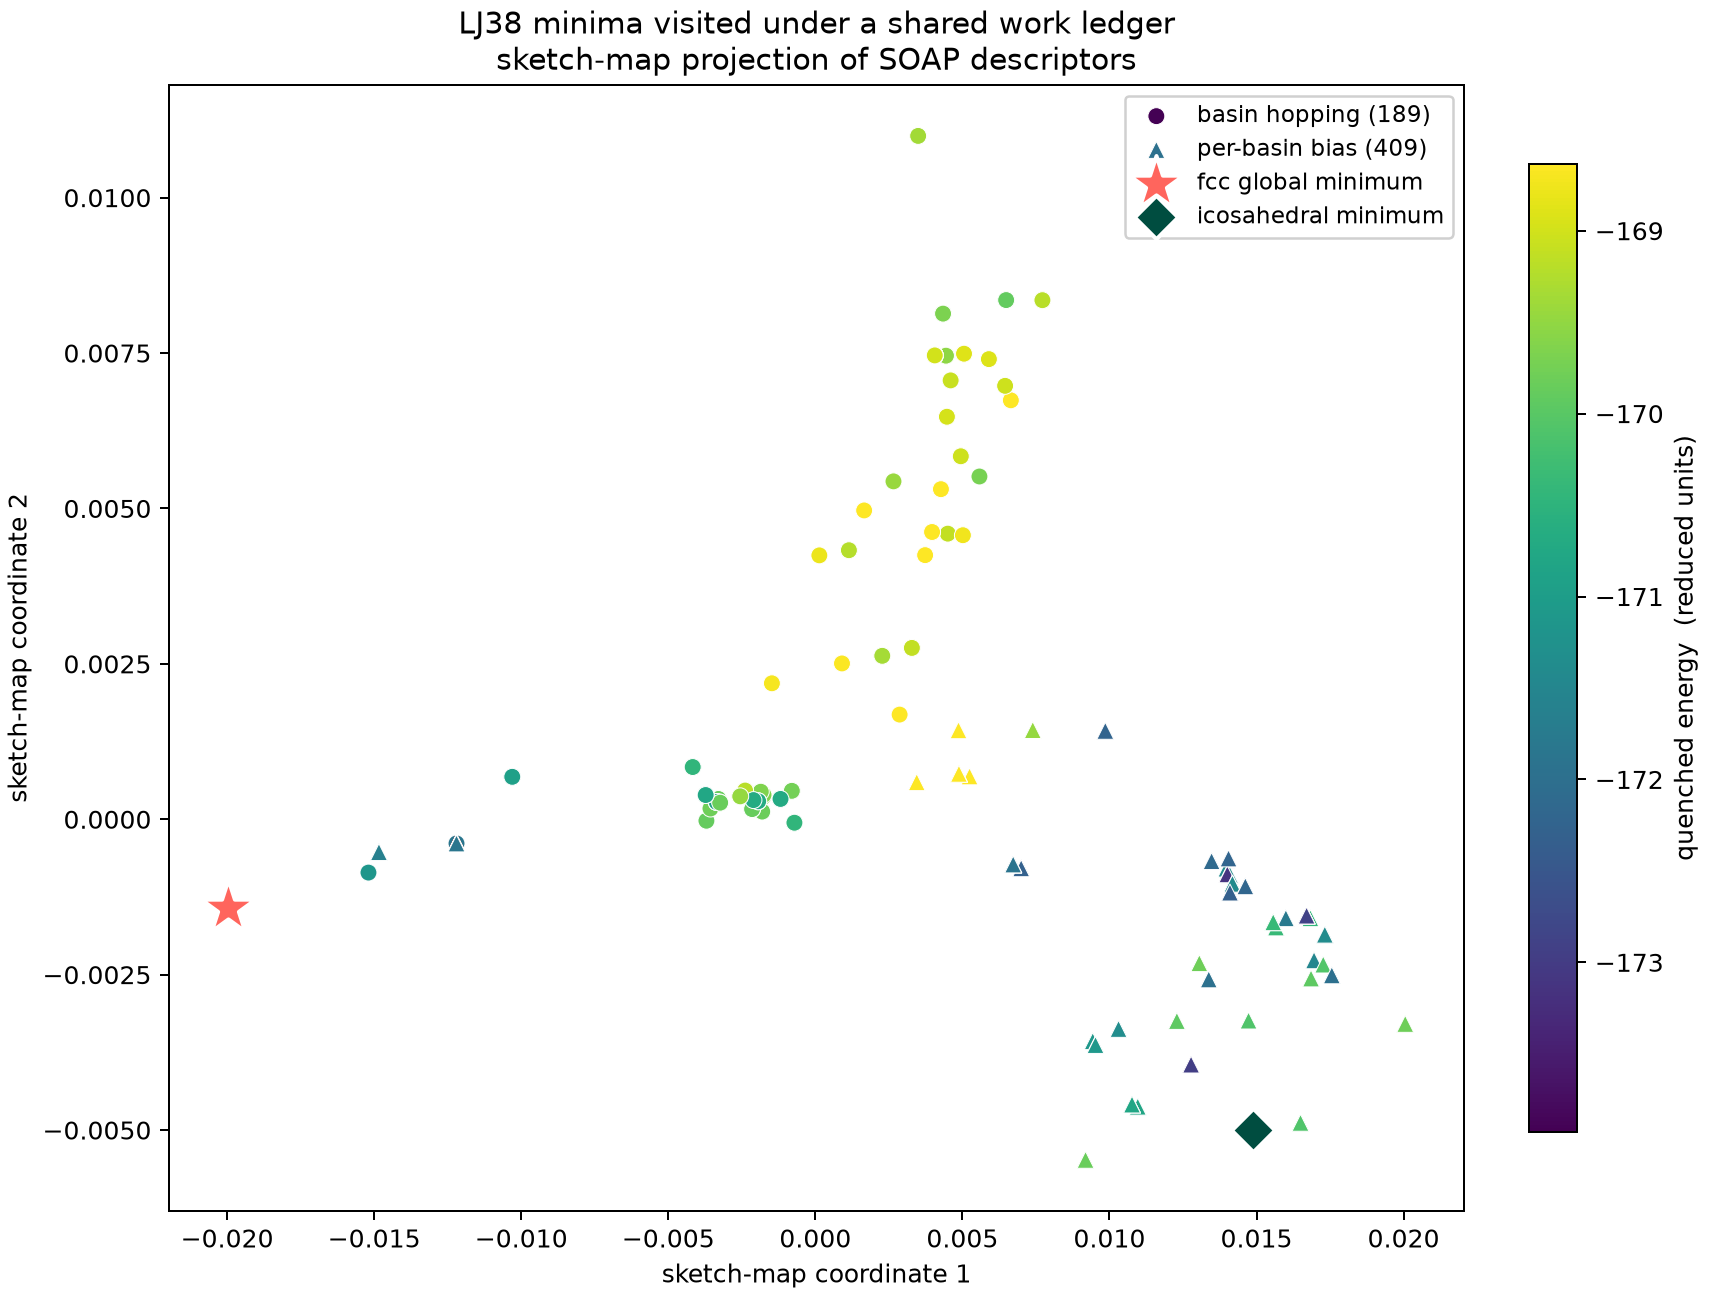
\includegraphics[width=0.48\textwidth]{lj38_sketchmap.png}
\caption{\(\mathrm{LJ}_{38}\) sketch-map.\cite{ceriotti2011}
Colour is the quenched energy.}
\end{figure}
\begin{figure}
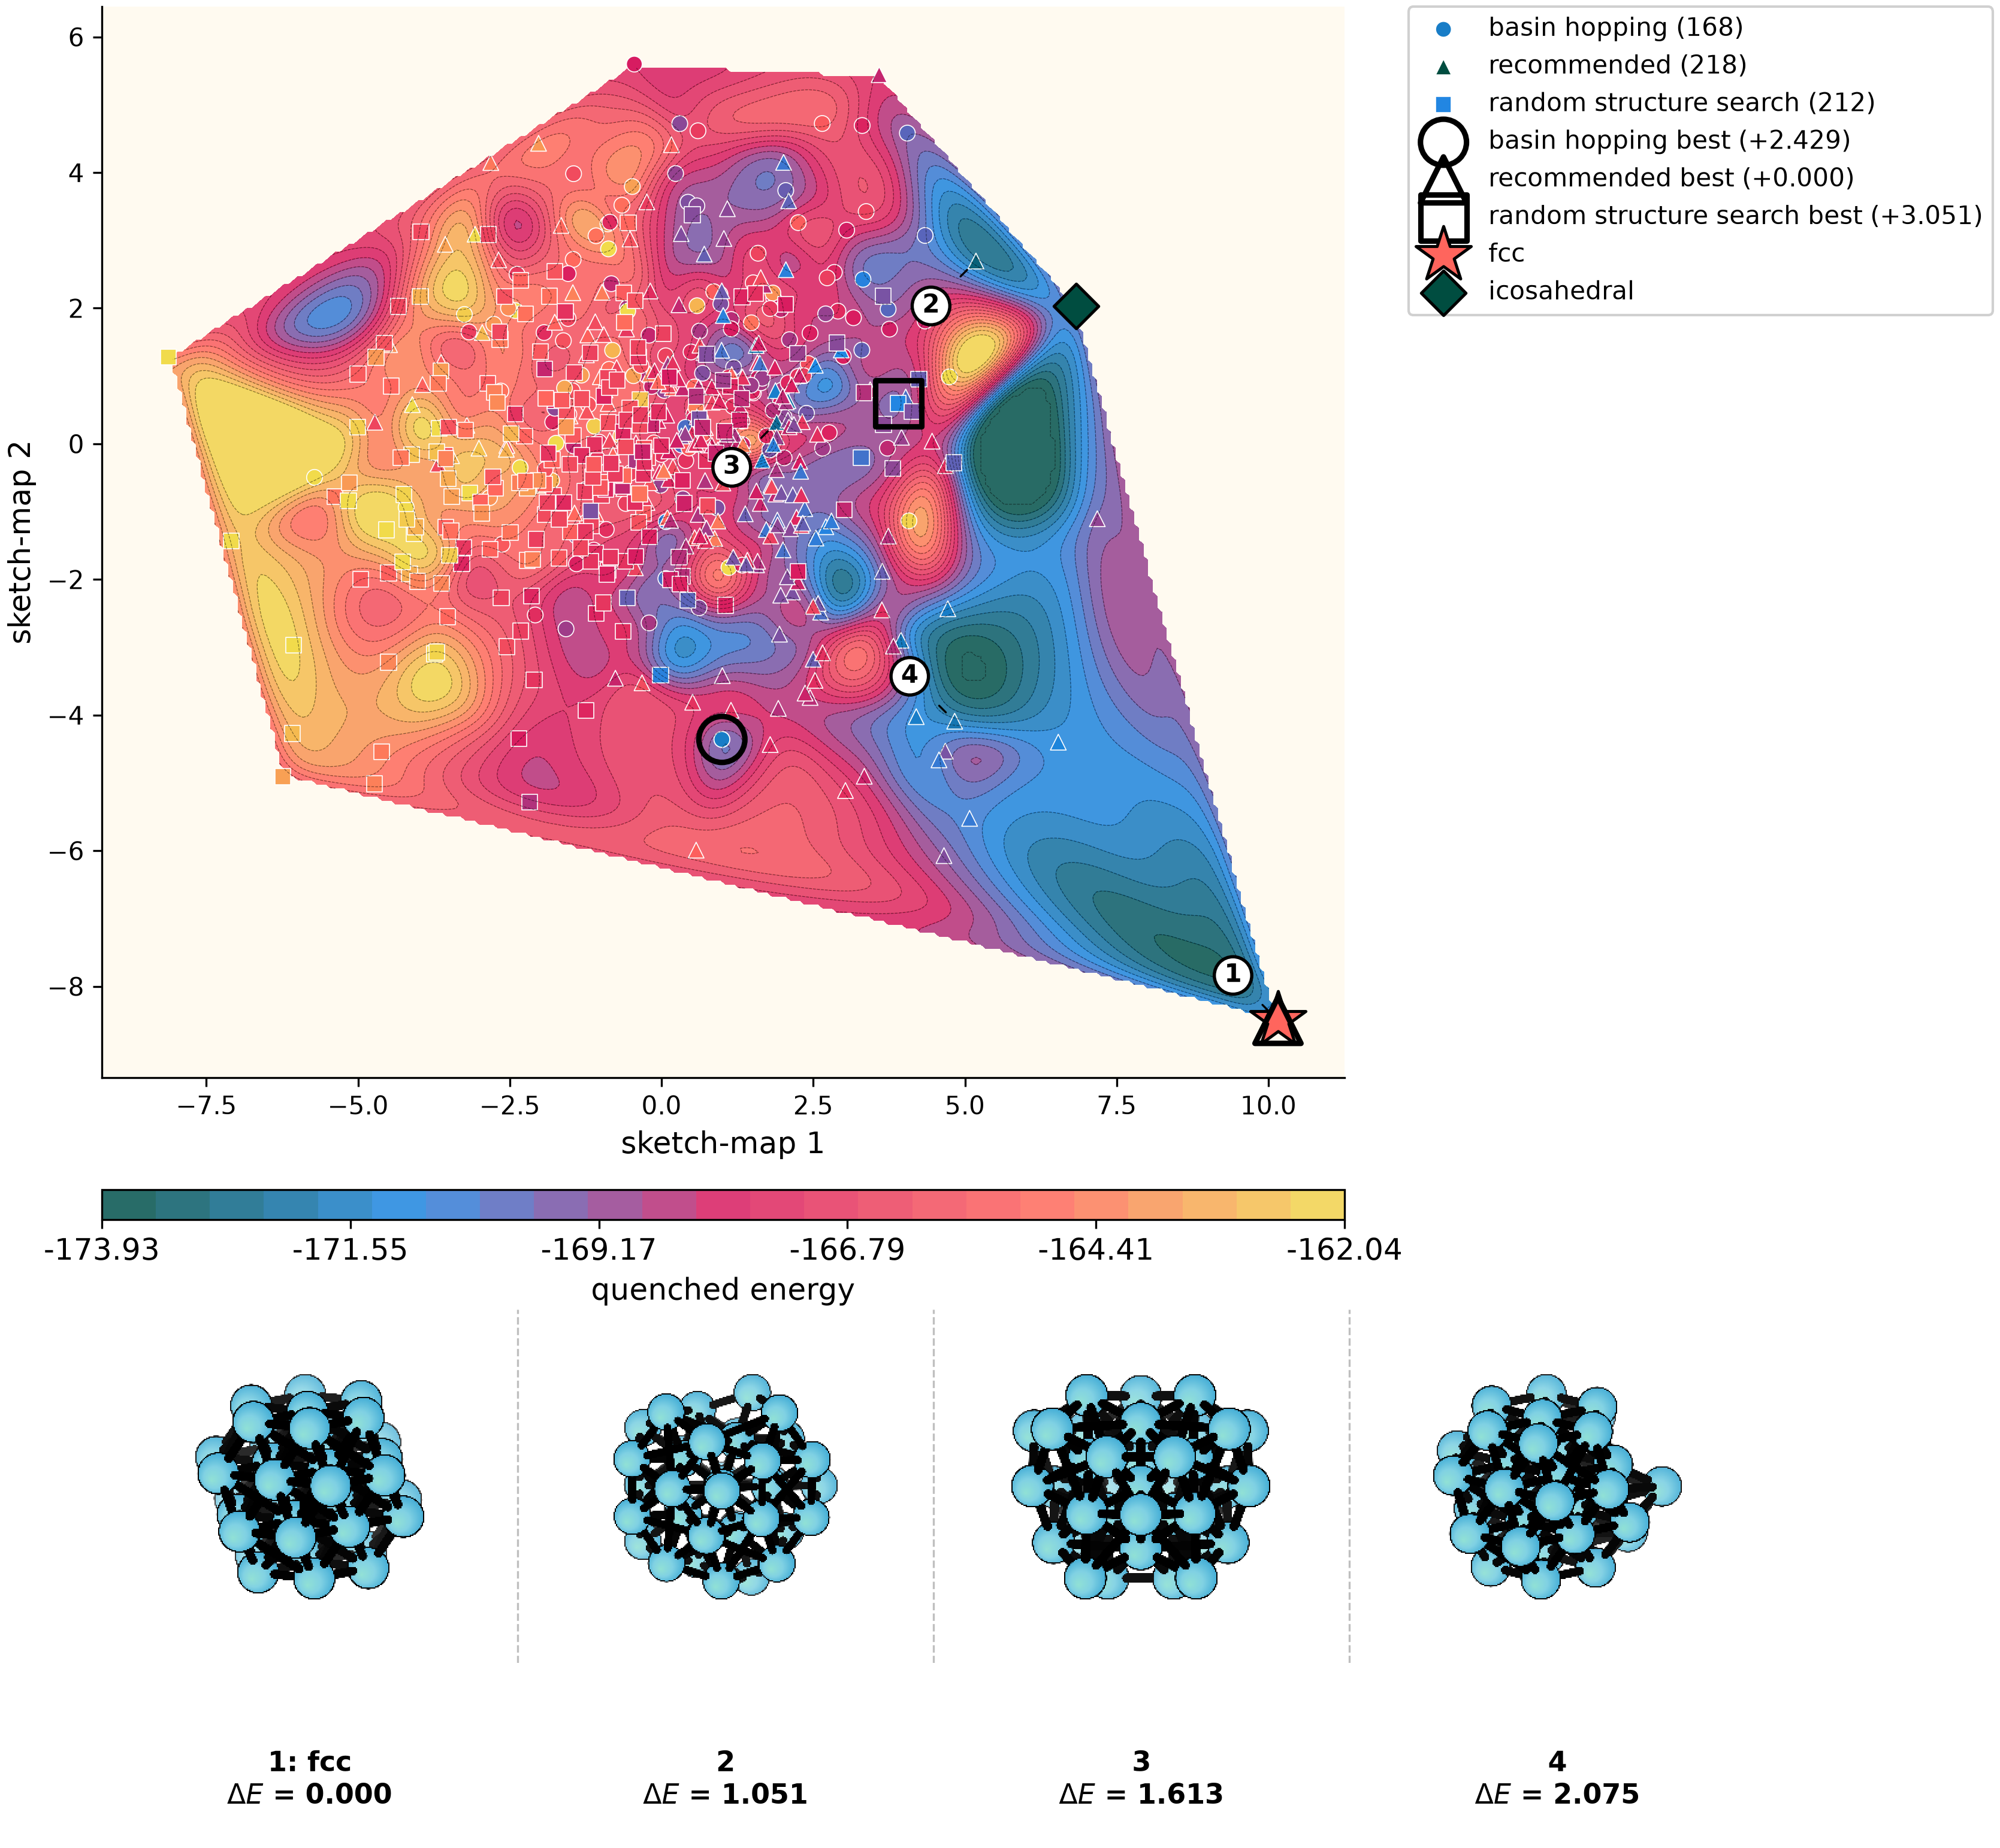
\includegraphics[width=0.48\textwidth]{lj38_landscape.png}
\caption{\(\mathrm{LJ}_{38}\) landscape.
Colour is the energy above the global minimum.
Basin hopping sits \(2.429\,\varepsilon\) above it and random structure search \(3.051\,\varepsilon\) above it.}
\end{figure}
\begin{figure}
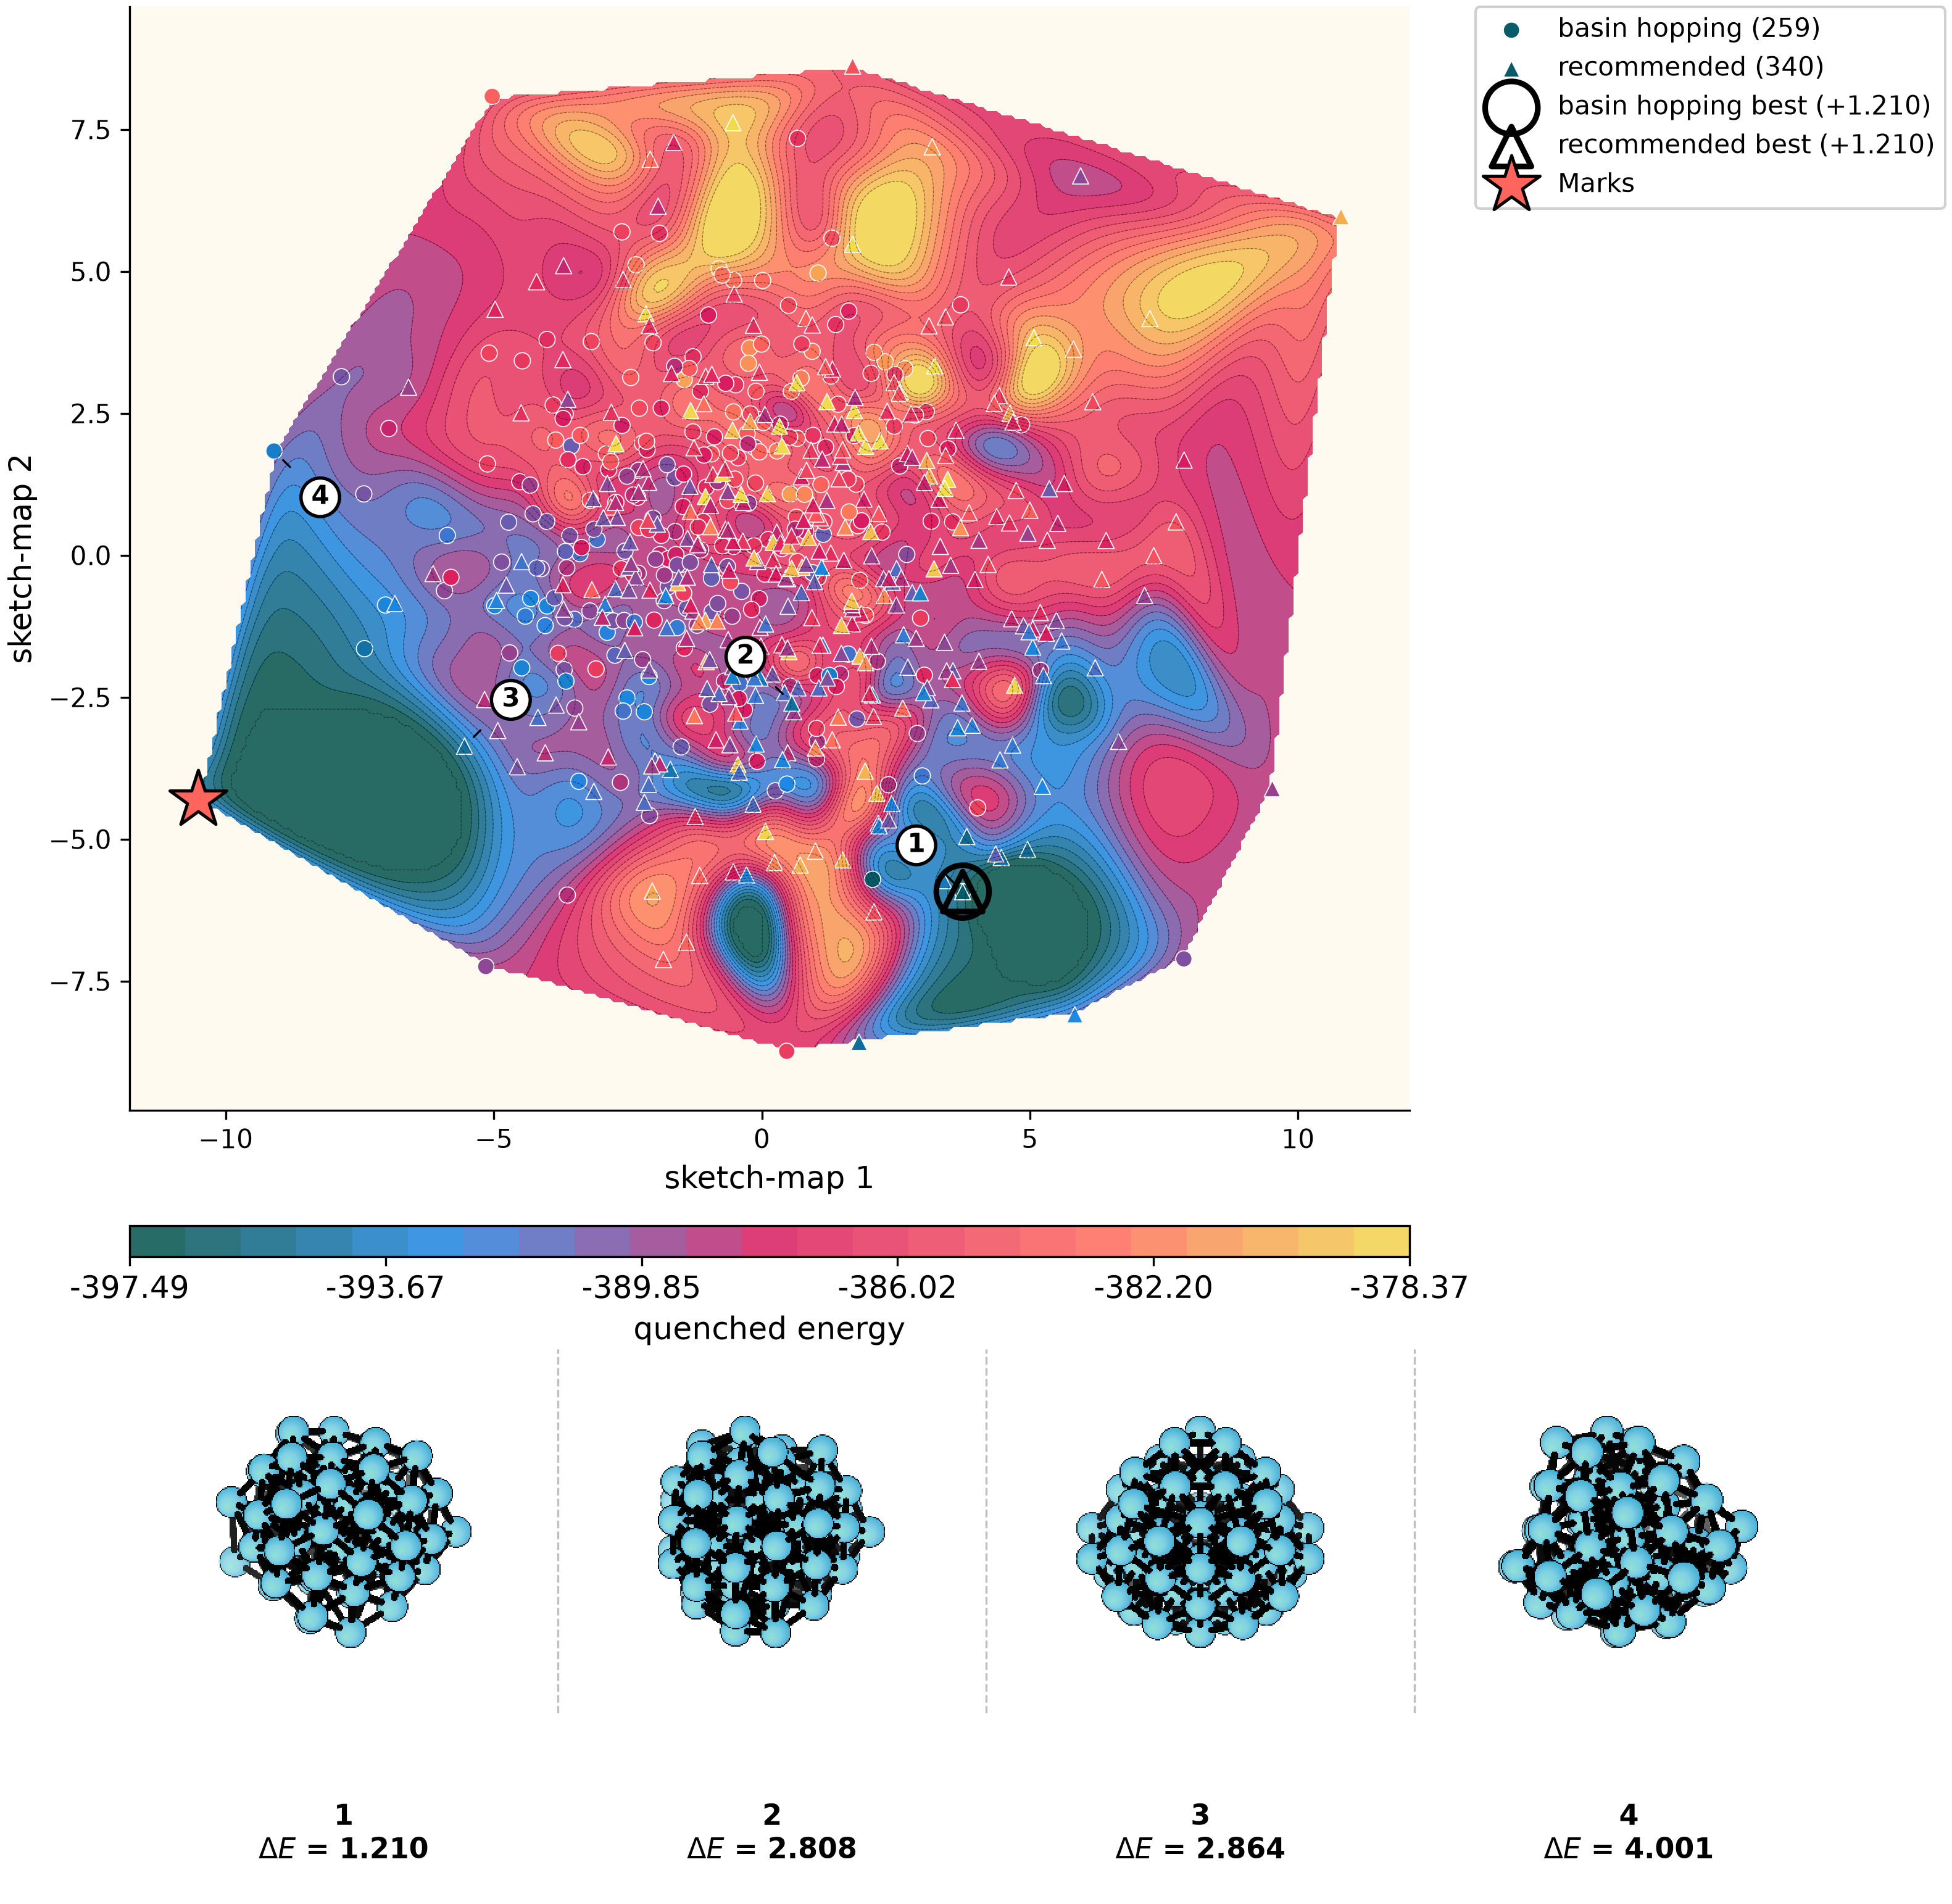
\includegraphics[width=0.48\textwidth]{lj75_landscape.png}
\caption{\(\mathrm{LJ}_{75}\) landscape.
Both arms sit \(1.210\,\varepsilon\) above the Marks decahedron.}
\end{figure}
\begin{figure}
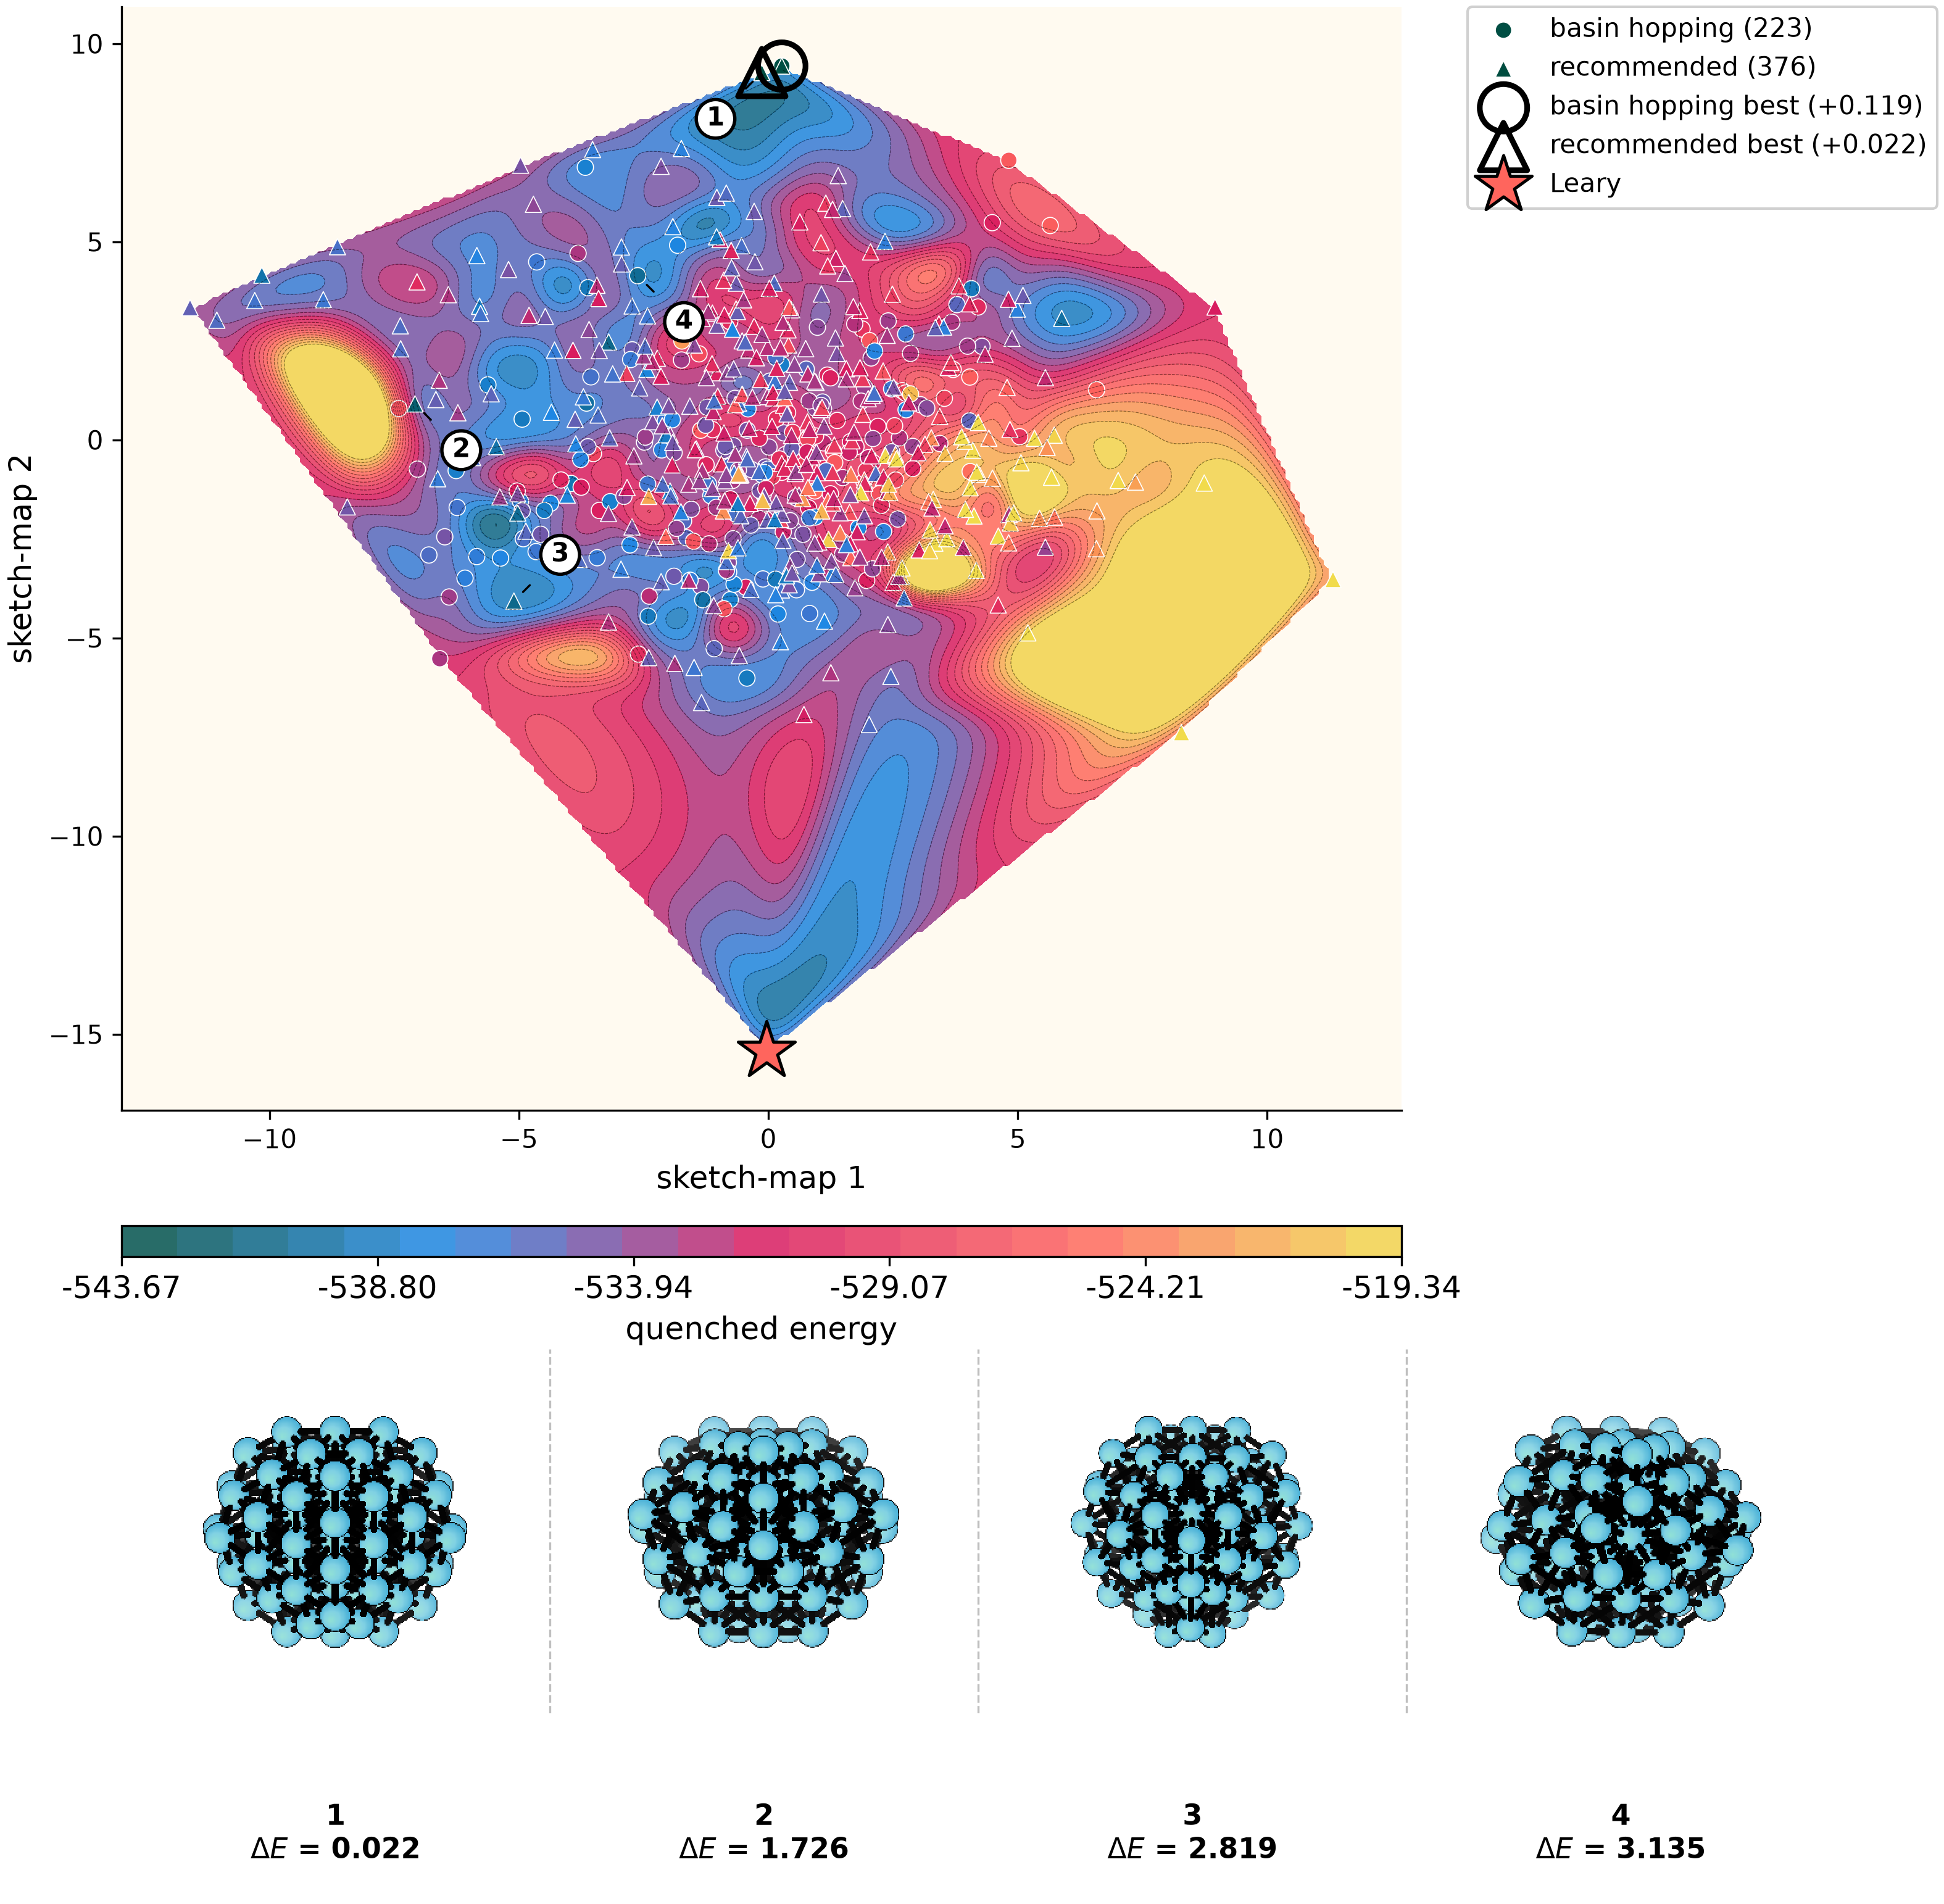
\includegraphics[width=0.48\textwidth]{lj98_landscape.png}
\caption{\(\mathrm{LJ}_{98}\) landscape.
The recommended hop sits \(0.022\,\varepsilon\) above the Leary minimum and basin hopping \(0.119\,\varepsilon\) above it.}
\end{figure}

One 38-atom walk with climb and symmetrisation off, seed 0 and 30000 charged evaluations, reaches \(-173.928427\).

\bibliographystyle{aipnum4-2}
\bibliography{../jctc/refs}

\end{document}
